\documentclass[11pt, a4paper]{elegantpaper}
\usepackage[utf8]{inputenc}
\usepackage{pgfplots}
\pgfplotsset{compat=1.18, width=10cm}
\usepackage{graphicx}
\graphicspath{ {./images/} }
\title{PANDANITE}
\author{Panda TEAM\thanks{founder Mr. Panda Bear}}
\date{February 2023}
\begin{document}
\maketitle

\section{Introduction}
Pandanite is a minimalist implementation of a layer-1 crypto-currency similar to Bitcoin. Pandanite is
designed with utmost simplicity, performance, and user friendliness in mind and is written from the
ground up in C++. Our hope is that Pandanite will be a more portable and lighter weight codebase
than Bitcoin, enabling Pandanite nodes to run on a broad range of low-cost devices yielding a
democratized network that is both fast-growing and expansive
\section{Circulation}
Pandanite is minted by miners who earn rewards. Mining payments occur using the following
algorithm, which yields a total final circulation of 100M PDN:
\begin{itemize}
	\item 50 PDN per block until block 666666
	\item $50*(2/3)$ PDN per block from blocks 666667 to 2*666666
	\item $50*(2/3)^2$ PDN per block from blocks 2*66666+1 to 3*666666 etc.
\end{itemize}
\begin{figure}[!h]
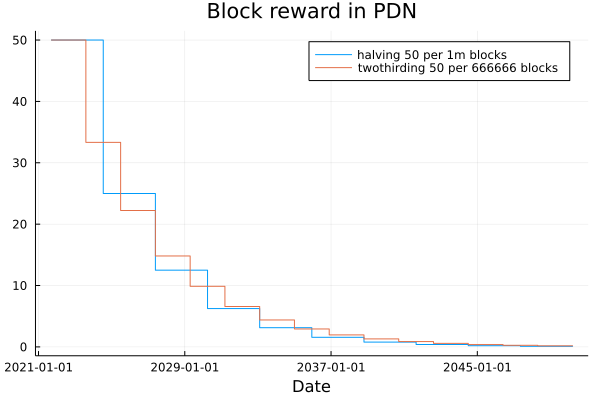
\includegraphics[width=8cm]{reward}
\centering
\caption{The payout curve is smoother in twothirding compared to halving:}
\end{figure}
\begin{figure}[!t]
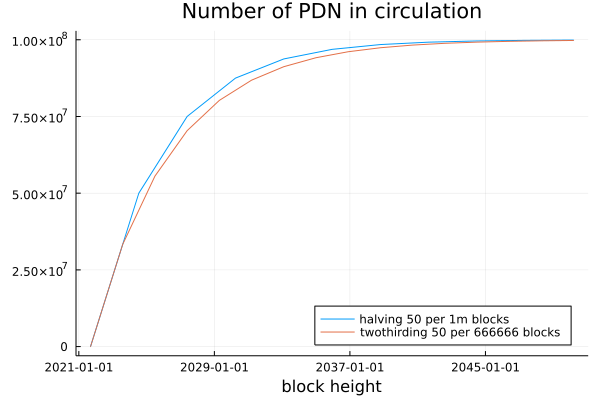
\includegraphics[width=8cm]{circulation}
\centering
\caption{Block reward changes are more often and have less impact compared to halving.}
\end{figure}
\section{Core Objectives}
Pandanite coin is intended to do as few things as possible and to do them incredibly well – it is a
store of value coin that:
\begin{itemize}
	\item Maintains account balances for billions of users.
	\item Provides extremely fast transactions between these accounts.
	\item Runs on low-cost hardware.
\end{itemize}
That’s it. We don’t aim to solve everything. We desire to keep the code simple.
\section{Implementation}
Pandanite is written in less than 6K lines of code (Bitcoin has >100K). There are a few optimizations
that we have made to help further our core objectives:
\begin{itemize}
	\item Switched encryption scheme from secp256k1 (which is used by ETH \& BTC) to ED25519 -- results in 8x speedup during verification and public keys half the size.
	\item 25,000 transactions per block
	\item 90 seconds block time
	\item SHA-256 based proof of work
\end{itemize}
Each block can contain between 1 and 25,000 transactions. The single transaction that is
required is the block mining fee paid out to the miner wallet.
\begin{figure}[h]
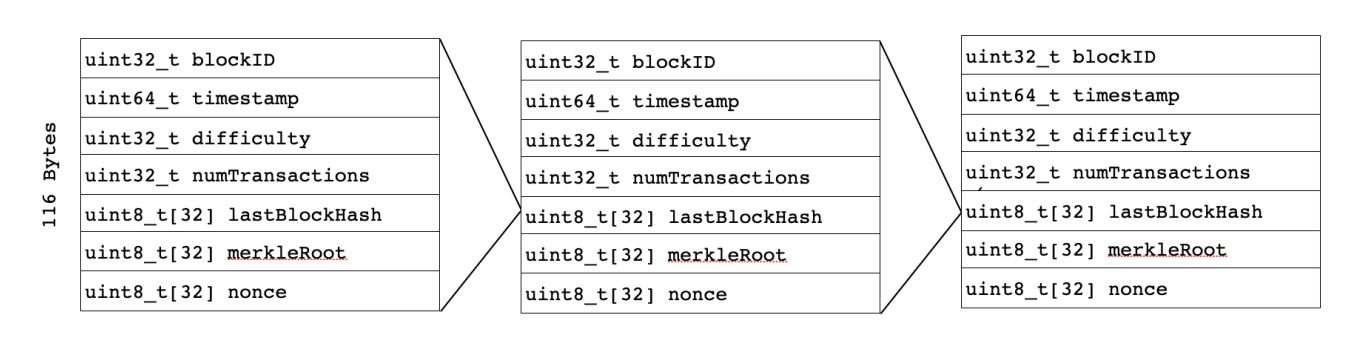
\includegraphics[width=\textwidth]{fig1}
\centering
\caption{The basic structure of the blockchain is almost identical to Bitcoin}
\end{figure}
\begin{figure}[h]
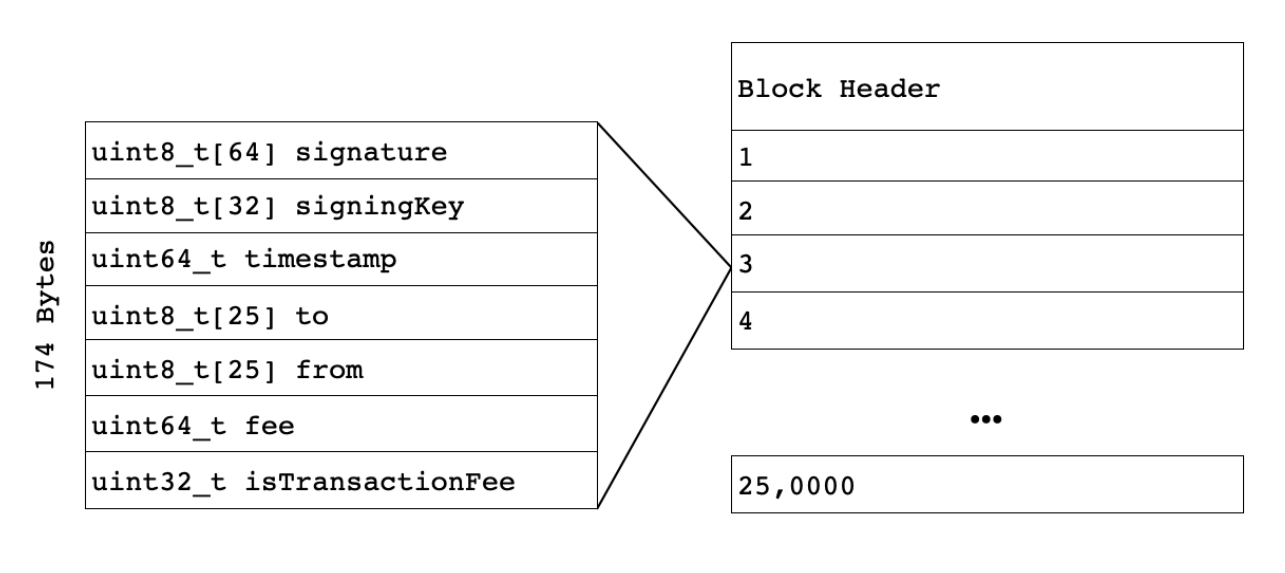
\includegraphics[width=\textwidth]{fig2}
\centering
\caption{There are up to 25,000 transactions in a single block}
\end{figure}

\section{Account Representation}
Each node stores a ledger containing a mapping between the wallet address (25 bytes) and the
total balance (8 bytes). This means each gigabyte of diskspace supports roughly 30 million users.
Furthermore the nodes store a list of all previously seen transaction hashes (32 bytes each) in order
to verify that submitted transactions have not executed in the past. For 1 million blocks at full
capacity this represents roughly 800 GB of disk space.
\section{Digital Signitures}
A key design objective of Pandanite is low compute usage while maintaining a high number of
transactions per second. To reach these performance goals Pandanite uses an alternative digital
signature system known as ED25519 as a replacement for Bitcoin and Ethereum’s secp256k1.
ED25519 has several attractive properties for crypto-currency use cases:
\begin{itemize}
	\item Fast signiture verification
	\item Batch signiture verification
	\item Fast signing
	\item Small public keys
	\item Performant on low-cost IoT devices
\end{itemize}
The first iteration of Pandanite utilizes the ref10 implementation of ED25519, which will be replaced
with a higher performance custom implementation supporting features like batch verification as
the network scales. To provide insight into the performance characteristics we provide comparisons
between Rust implementations of ED25519 against a Rust wrapper of Bitcoin’s native libsecp256k1.
\begin{figure}[h]
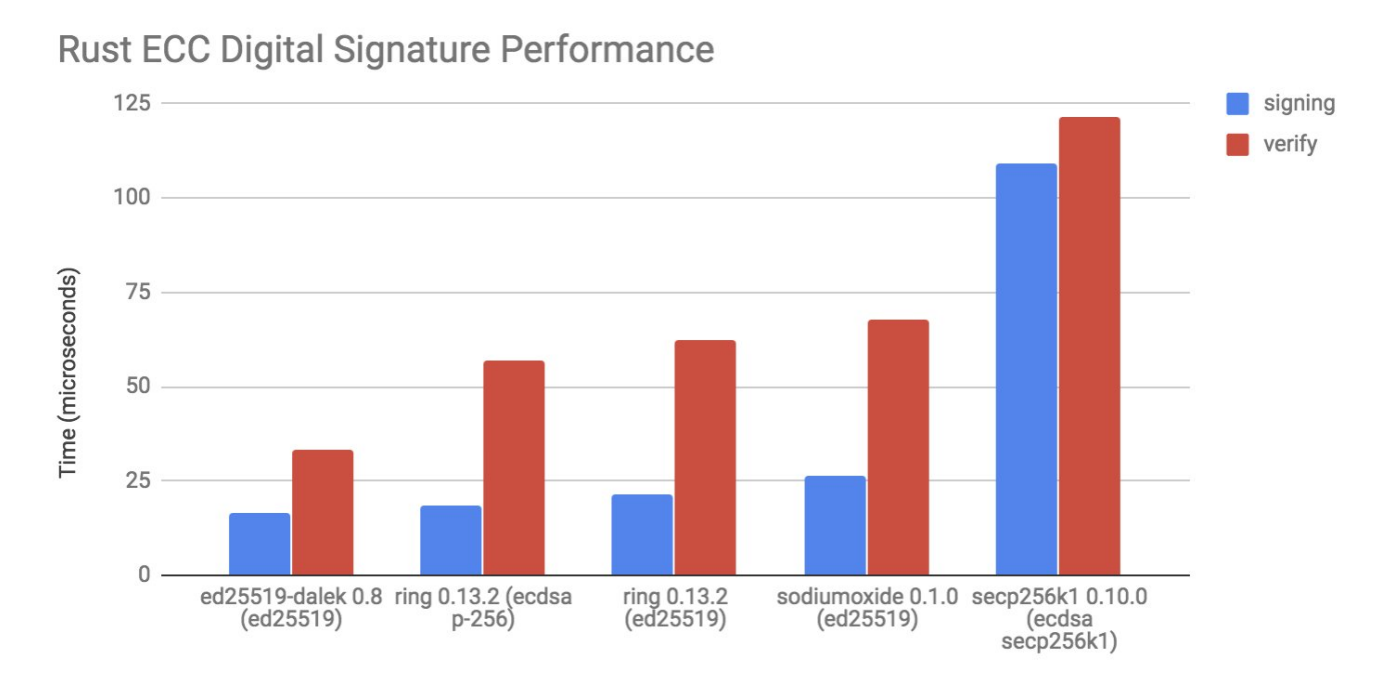
\includegraphics[width=\textwidth]{fig3}
\centering
\caption{Performance comparison of digital signature algorithm implementations}
\end{figure}
\section{ Proof Of Work}
Pandanite uses a simple proof of work scheme based on SHA256 and Pufferfish 2 $(P)$. Given a block
header $B$ and it’s hash $H = \text{SHA 256}(B)$ the miner must provide a 256-bit nonce $N$ such that
SHA 256$(P(H||N))$ has a minimum of $k$ leading zero bits, where $k$ is a difficulty parameter.
\begin{equation}
\gamma(\text{SHA 256}(P(H||N)))\,>\,k
\end{equation}
Difficulty is then measured in bits and the number of hashes expected prior to finding a valid nonce at difficulty $k$ is simply $2^k$. Difficulties adjust every 100 blocks based on the ratio of elapsed to expected time. Pufferfish 2 is an ASIC resistant memory hard hash function developed for the password hashing competition by Jeremi M. Gosney.
\section{Performance}
Pandanite coin is designed to support a peak rate of 250 transactions per second (tps), significantly
greater than Bitcoin (7 tps) or Ethereum (15 tps). This is due to a larger block size than Bitcoin’s
(4.35 MB vs 1MB) and shorter block mint time (90 sec vs. 600 sec). We believe that faster internet
connections in 2021 than 2010 will enable us to push these fixed limits without yielding an excess
number of forks in the network.
\section{ Roadmap}
The Pandanite project timeline:
\begin{itemize}
	 \item 2022 FEB: Pandanite (PDN) launched, formerly known as Bamboo (BMB)
	\item 2022 DEC: rebrand completed 
	\item 2023 JAN: faster node synch achieved and "twothirding" implemented"
	\item 2023 FEB: Site 2 deployed
	\item 2023 Q1-Q2: new explorer ( @CoinFuMasterShifu ) and some minor changes
	\item 2023 Q3: "twothirding" event happens
\end{itemize}
Rest of 2023 and beyond:
Continuous work:
\begin{itemize}
\item wallet development
\item code clean up/fix
\item additional node development
\item website polish
\item stimulating organic growth
\item achieving new partnerships
\end{itemize}
\section{Conclusion}
We have presented our vision for Pandanite: a minimal and elegant layer-1 crypto-currency codebase
that can do basic transactions quickly and efficiently for billions of users across a broad number
of devices. It is our hope that Pandanite code will always be compact and clear enough that even
novice programmers will be able to modify and improve Pandanite. For more information please
visit us on:
\begin{itemize}
\item \href{https://github.com/pandanite-crypto}{Github}
\item \href{https://bitcointalk.org/index.php?topic=5428374.0}{Bitcointalk}
\item \href{https://discord.com/invite/crfkWjxYyT}{Discord}
\item \href{https://twitter.com/pdn_pandanite}{Twitter}
\item \href{https://t.me/pandanite}{Telegram}

\end{itemize}



\end{document}
